\documentclass{article} %A4
\usepackage[a4paper,left=1.9cm, right=2.1cm,top = 1.2cm,bottom=2.3cm]{geometry}
\usepackage[utf8]{inputenc}%Umlaute
\usepackage[ngerman]{babel} %Texttrennung
\usepackage{graphicx}	%Grafiken
\usepackage{amssymb}
\usepackage{amsmath}
\usepackage{amsthm}
\usepackage{url}
\usepackage{listings}
 \usepackage{color}
\usepackage{hyperref}
\usepackage{framed}
\usepackage{algpseudocode}
\usepackage{tikz}
\usepackage{sgame}
\usepackage{multicol}
\usepackage[labelformat=empty]{caption}

\title{Zusammenfassung - Multi-Agenten-Systeme}
\author{
	Andreas Ruscheinski,
	Marc Eric Meier, 
	CD
}
\begin{document}
\maketitle
\begin{framed}Korrektheit und Vollständigkeit der Informationen sind nicht gewährleistet.
Macht euch eigene Notizen oder ergänzt/korrigiert meine Ausführungen!
\end{framed}
\setcounter{tocdepth}{1}
\tableofcontents

\section{Einführung}
	\subsection{Definition}
	\begin{itemize}
		\item Ein Agent ist ein Computer System, welches \textbf{selbstständig} Aktionen im Interesse des Benutzers ausführen kann.
		\item Ein Agent \textbf{befindet} sich in einer \textbf{dynamischen Umgebung}, mit welcher er interagiert.
		\item Ein Multi-Agenten-System besteht aus \textbf{mehreren Agenten}, welche \textbf{miteinander interagieren}.
		\item In einem Multi-Agenten-System ist es für eine  \textbf{erfolgreiche Interaktion} notwendig, dass die Agenten miteinander \textbf{kooperieren}, \textbf{verhandeln} und \textbf{sich abstimmen} können.
	\end{itemize}
	\subsection{Eigenschaften}
	\begin{itemize}
		\item Jeder Agent hat \textbf{keine vollständigen Informationen} über die Umgebung.
		\item Es gibt \textbf{keine globale Kontrolle} der Agenten.
		\item Die Daten sind \textbf{dezentralisiert}.
		\item Die Berechnung erfolgt \textbf{asynchron}.
	\end{itemize}
	\subsection{Gründe für den Einsatz von MAS}
	\begin{itemize}
		\item Ein Problem kann nicht zentralisiert gelöst werden, da die \textbf{Ressourcen limitiert} sind.\\
		$\rightarrow$\textit{Verteilte Berechnungen}
		\item \textbf{Reduktion der Ausfall-Wahrscheinlichkeit} gegenüber einem zentralisierten System
		\item \textbf{Gewährleistung der Interkonnektion und Interoperation} von verschiedenen Systemen\\
		$\rightarrow$\textit{Migration von veralteter Software}
		\item Lösung von Problemen, die sich mit einer \textbf{ Menge von autonomen Komponenten beschäftigen}\\
		$\rightarrow$\textit{Luftfahrkontrolle, Terminkalender}
	\end{itemize}
	\subsection{Konkrete Anwendungsgebiete}
	\begin{itemize}
		\item Cloud-Management
		\item Ubiquitous Computing
		\item Grid-Software
		\item Spiele
		\item Verschiedene Gebiete der Industrie (Car-Assembly, Factory Management)
		\item Simulation
	\end{itemize}
	MAS befindet sich in der Schnittmenge aus KI, Spieltheorie, Sozialforschung und Verteilten Systemen.
\section{Rolle der Logik in MAS}
	\subsection{Gründe für Logik}
	\begin{itemize}
		\item Wissensbasis + Aktionen mit Voraussetzung und Auswirkung $\rightarrow$ Plan für Lösung des Problems
		\item Verwaltung von Annahmen
		\item Logik ist ein Framework für das Verstehen von Systemen
		\item Verifikation, Ausführungsspezifikation, Planung
		\item Agenten als Theorembeweiser
	\end{itemize}
	\subsection{Logik-basierende Architektur}
	\begin{itemize}
		\item Grundidee: Aufstellen einer Regelmenge zur Beschreibung der besten Aktion bei einem gegebenem Zustand
		\item Bestandteile:
		\begin{itemize}
			\item $p$: Eine Theorie (Menge von Regeln)
			\item $\Delta$: Datenbank mit dem aktuellen Zustand der Welt
			\item $A$: Eine Menge von Aktionen, die ein Agent ausführen kann
			\item $\Delta\vdash_{p}\phi$: d.h. $\phi$ kann aus der $\Delta$ unter der Verwendung von $p$ abgeleitet werden, mit $\phi=$Do(a) können wir aus dem aktuellen Zustand der Welt auf die bestmögliche Aktion logisch schließen.
		\end{itemize}
		 \item Algorithmus-Bestandteile (unabhängig von einer verwendeter Logik)
		 \begin{itemize}
		 	\item \textbf{see(s,p)}, generiert Beobachtung aus der aktuellen Welt $s$ (schwer siehe Vorlesung Mustererkennung und Kontextanalyse)
		 	\item \textbf{next($\Delta$,p)}, Update der Datenbank mit der Beobachtung
		 	\item \textbf{action($\Delta$)}, ermittelt die auszuführende Aktion aus der Datenbank, entweder ist die Aktion direkt beschrieben oder kann aus den Regeln abgeleitet werden.
		 \end{itemize}
		 \item Algorithmus - Ermittelung einer Aktion aus einer Wissensdatenbank:
		 \begin{enumerate}
		 	\item Überprüfe für jede Aktion a, ob  $\Delta\vdash_{p}Do(a)$ gilt (d.h. a kann direkt abgeleitet werden)
		 	\item Falls ja: Gib a zurück; sonst
		 	\item Überprüfe für jede Aktion a, ob $\Delta\not{\vdash}_{p}\neg Do(a)$ gilt (d.h a ist nicht explizit ausgeschlossen)
		 	\item Falls ja: Gib a zurück, sonst gib NULL zurück (keine Aktion gefunden)
		 \end{enumerate}
	\end{itemize}
	\subsection{Modale Logik}
	\begin{itemize}
		\item Erlaubt Ausdrücke wie: wahrscheinlich wahr, geglaubt wahr, wahr in der Zukunft usw.
		\item Kann genutzt werden, um Informationen für die Agenten abzuleiten und über das Wissen von Agenten zu schließen
		\item Syntax:
		\begin{itemize}
			\item Prädikatenlogik mit Erweiterung
			\item Prop: Eine Menge von atomaren Formeln
			\item Wenn $p,q \in Prob$, dann sind auch $\neg p, p \& q, \diamond p,\square p$ Formeln
			\item $\diamond$ p: möglicherweise p, manchmal p 
			\item $\square$p: immer p, notwendigerweise p
		\end{itemize}
		\item Semantik:
		\begin{itemize}
			\item Kripke-Struktur: $\mathcal{K} = <W,R,\mu>$
			\begin{description}
				\item[$W$] eine Menge von Welten
				\item[$R$] eine Menge von binären Relationen, die den Übergang zwischen den Welten  beschreiben
				\item[$\mu$] Abbildungsfunktion, die jeder Welt Eigenschaften zuordnet ($\mu : W \rightarrow 2^{Prop}$)	
			\end{description}
				\item Rahmen: $<W,R>$
				\begin{itemize}
					\item  $W$ und $R$ definiert, wie in Kripke Struktur
					\item $R \vdash F$, falls gilt: $\forall \mathcal{K},s: \mathcal{K},s \vDash F$ 
					\item Die \textbf{Korrespondenztheorie}: Zusammenhang zwischen Axiomensystemen und Rahmen					
				\end{itemize}
			\item Definition von $\diamond$ und $\square$ Operator auf Basis von Erreichbarkeit der Welten in einer Kripke-Struktur
			\item $\square p$: p ist wahr in allen Welten, welche von der aktuellen Welt erreichbar sind
			\item $<M,w>\vDash\square p$, wenn für alle $w' \in W$ gilt: wenn $(w,w') \in R$ denn $<M,w'>\vDash p$
			\item $\diamond p$: p ist wahr, wenn mindestens eine Welt erreichbar ist, in welcher p wahr ist
			\item $<M,w>\vDash\diamond p$, wenn es ein $w' \in W$ existiert mit:  wenn $(w,w') \in R$ denn $<M,w'>\vDash p$\\
			
			\item Für R muss zusätzlich gelten:
			\begin{description}
				\item[reflexiv] für jedes $x \in W$ gilt $R(x,x)$, d.h. x ist von x aus erreichbar.
				\item[transitiv] für jedes $x,y,z \in W$ gilt $R(x,y) \wedge R(y,z) \implies R(x,z)$, d.h. wenn man von x nach y und von y nach z gehen kann, kann man auch von x nach z gehen.
				\item[seriell] für jedes $x \in W$ existiert ein $y$, so dass gilt $R(x,y)$, d.h. jede Welt ist mit einer anderen Welt in Relation.
				\item[euklidisch] wenn für jedes $x,y,z \in W$ mit $R(x,y)$ und $R(x,z)$, dann gilt auch $R(y,z)$, d.h. wenn man von x nach y und von x nach z gehen kann, dann kann man auch von y nach z gehen.\\
				
			\end{description}
			\begin{table}[h]
				\centering
				\label{my-label}
				\begin{tabular}{llll}
					\hline
					Name & Axiom                          & Condition on R & First-order characterization \\ \hline
					T    & $\square\phi \Rightarrow \phi$ & Reflexive      & $\forall w\in W:(w,w)\in R$  \\
					D & $\square\phi \Rightarrow \diamond\phi$ &        Serial        &$\forall w \in W : \exists w' \in W: (w,w')\in R$\\
					4&$\square\phi\Rightarrow\square\square\phi$ &            Transitive    & $\forall$ \\
					5 &$\diamond\phi\Rightarrow\square\diamond\phi$&     Euclidiean           &                              \\ \hline
				\end{tabular}
		\caption{Korrespondenztheorie}
			\end{table}
			\item Axiome (Beschreiben Eigenschaften für $R$):
			\begin{description}
				\item[$\square p \Rightarrow p$] Wann immer $p$ wahr ist, folgt daraus, dass aktuell p gilt (\textbf{Reflexiv})
				\item[$\square p \Rightarrow \diamond p$]Wann immer $p$ wahr ist, ist p auch in mindestens einer Welt wahr (\textbf{Seriell})
				\item[$\square p \Rightarrow \square \square p$]Wann immer $p$ wahr ist, ist p auch immer wahr, wenn wir einen Übergang machen (\textbf{transitiv})
				\item[$\diamond p \Rightarrow \square \diamond p$] Wenn $p$ in mindestens einer Welt wahr ist, ist p für immer wahr, wenn wir diese Welt erreicht haben (\textbf{euklidisch})\\
				
			\end{description}
			
			\item Anwendung der Modal Logik auf Agenten durch Einführung von Indizes, welche entsprechend für Agent gelten
			\item Operator - Knowledge: $K_ip$ bedeutet, dass Agent i $p$ weiß
			\item Der Modale Operator $\square_i$ wird zu $K_i$\\
			
			\item Axiome und Agenten:
			\begin{description}
				\item[$K_{i}p \Rightarrow p$] Wenn Agent glaubt, dass p wahr ist, ist p auch in Wirklichkeit wahr
				\item[$K_{i}p \Rightarrow \neg K_{i}\neg p$] Wenn Agent glaubt, dass p wahr ist, glaub er nicht die Negation
				\item[$K_{i}p \Rightarrow K_{i}K_{i}^p$] Wenn Agent glaubt, dass p wahr ist, weiß er selbst, dass er p glaubt
				\item[$\neg K_{i}\neg p \Rightarrow K_{i}\neg K_{i}\neg p$] Wenn der Agent nicht p glaubt, weiß er dass er nicht p glaubt.\\
				
			\end{description}
			\item Es gilt: $<M,w> \vDash K_i p$, genau dann wenn $\forall w' \in W$ gilt: wenn $(w,w') \in R_i$, dann $<M,w'> \vDash p$ (vgl. Definition von $\square$)
			\item Probleme:
			\begin{itemize}
				\item Agent glaubt alles was wahr ist incl. Tautologien: wenn $\vDash p$ denn $K_i p$
				\item Agent weiß alle Schlussfolgerungen des eigenen Wissens: $\vDash p \rightarrow q$ denn $\vDash K_i p \rightarrow K_i q$ (Kripke Axiom: $K_i(p\rightarrow q) \rightarrow (K_i p \rightarrow K_i q)$)
				\item Menschliches Wissen ist oft inkonsistent
				\item Menschen glauben nicht alle äquivalenten Aussagen
			\end{itemize}
		\end{itemize}
	\end{itemize}
	\subsection{BDI-Logic}
	\begin{description}
		\item [Beliefs]
			\begin{itemize}
				\item \textbf{Aktuelles Weltwissen} inklusive Umgebungszustand und internem Wissen
				\item \textbf{Informationskomponente} über Systemzustand
			\end{itemize}
		\item[Desires] 
			\begin{itemize}
				\item Beschreiben den \textbf{Zustand, den ein Agent zu erreichen versucht}
				\item Kann als \textbf{Anregungszustand des Systems} betrachtet werden
			\end{itemize}
		\item[Intentions]
			\begin{itemize}
				\item \textbf{Der gewählte Weg} eines Agenten um seine Desires zu erreichen.
				\item Intention beschreibt die Komponente zur \textbf{Entscheidungsfindung} des Agenten
				\item \textbf{Committment} beschreibt Grad der Festlegung auf eine Aktionsausführung
			\end{itemize}
	\end{description}
	
	\begin{itemize}
		\item Klassische logische Operatoren: und, oder, Negation usw...
		\item CTL* Path Quantifikatoren (Computation Tree Logic)
		\begin{itemize}
			\item $A \phi$: es gilt auf allen Pfaden $\phi$
			\item $E \phi$: es gilt auf einigen Pfaden $\phi$
			\item $G$: global
			\item $F$: zukünftig
		\end{itemize}
		\item BDI-Funktionen:
		\begin{itemize}
			\item (Bel i $\phi$): i glaubt $\phi$
			\item (Des i $\phi$): i will $\phi$
			\item (Int i $\phi$): i verfolgt $\phi$
		\end{itemize}
		\item Regeln:
		\begin{itemize}
			\item (Des $\alpha$) $\rightarrow$ (Bel $\alpha$) (Belief goal compatibility): Wenn der Agent $\alpha$ erreichen will, folgt daraus, dass der Agent an die Machbarkeit von $\alpha$ glaubt.
			\item (Int $\alpha$) $\rightarrow$ (Des $\alpha$) (Goal-intention compatibility): Wenn der Agent $\alpha$ verfolgt, folgt daraus, dass der Agent $\alpha$ erreichen will.
			\item (Int does(a)) $\rightarrow$ does(a) (Volitional commitment): Wenn der Agent does(a) ausführen möchte, wird er diese als nächstes ausführen.
			\item (Des $\alpha$) $\rightarrow$ (Bel (Des $\alpha$)) und (Int $\alpha$) $\rightarrow$ (Bel (Int $\alpha$)) (Awareness of goals \& intentions): Bedingt, dass neue Ziele und Intentionen als Event gepostet werden, müssen in der Wissensbasis...
%TODO Satz vervollständigen -> müssen in der Wissensbasis....
			\item done(a) $\rightarrow$ (Bel (done(a))) (No unconscious actions): Wenn ein Agent eine Aktion ausgeführt hat, weiß er, dass er diese ausgeführt hat.
			\item (Int $\alpha$) $\rightarrow$ AF($\neg$(Int $\alpha$)) (No infinite deferral): Ein Agent will eine Intention verfolgen oder diese verwerfen.
		\end{itemize}
		\item reaktive und proaktive Agenten
		\begin{itemize}
			\item Reaktiv: Aktion wird ausgeführt durch eine Eingabe: Wenn Eingabe = p denn tu a
			\item Proaktiv: Planung und Ausführung von Aktionen, um ein Ziel zu erreichen: Tu a, um p zu erreichen
		\end{itemize}
	\end{itemize}
	
\section{Planning}
	\subsection{Einführung - Brooks Vision}
	\begin{itemize}
		\item Ziel 1: Intelligentes Verhalten ohne explizite Repräsentation von Wissen
		\item Ziel 2: Intelligentes Verhalten ohne abstraktes Schließen über die Repräsentation des Wissens
		\item Idee 1: Echte Intelligenz gibt es nur ein einer Welt und nicht losgelöst von dieser wie, in Theorem Beweisern und Expertensystemen
		\item Idee 2: Intelligentes Verhalten entsteht erst als Ergebnis der Interaktion mit der Umgebung
	\end{itemize}
	\subsection{Subsumption Architektur}
	\begin{itemize}
		\item Traditionell: Die Intelligenz steht zwischen Beobachtung und Aktion, d.h. aus Beobachtungen wird geschlossen welche Aktion ausgeführt wird.
		\item Neu: Die Intelligenz entsteht beim Beobachter durch die Aktionen in der Welt, d.h. ein Agent ist nicht an sich intelligent, sondern wirkt intelligent für einen Beobachter
		\item Entscheidungsfindung durch verschiedene Aufgaben:
		\begin{itemize}
			\item Verhalten ist eine Abbildung von Zustand auf Aktion
			\item Verarbeitung der Sensorwerte mit Schluss auf den Zustand
			\item Zustände und Aktionen sind direkt gekoppelt
		\end{itemize}
		\item Mechanismus zur Auswahl der Aktionen: Prioritäten  $\rightarrow$ d.h Verhalten mit hoher Priorität kann Verhalten mit niedrigeren Prioritäten unterdrücken
		\item Formales Modell:
		\begin{itemize}
			\item Ein Verhalten (Behavior) $b \in Beh$ ist ein Tupel $(c,a)$ mit $c \subseteq P, a \in A$ wobei P eine Menge von Beobachtungen und A eine Menge von Aktionen ist.
			\item Ein Verhalten wird ausgeführt, wenn die Umgebung sich in dem Zustand $s\in S$ befindet und $see(s) \in c$
			\item Subsumption Hierarchie wird realisiert durch eine Hemmungs-Relation $b_{1} \prec b_{2}$ ($b_{1}$ hemmt $b_{2}$ d.h. $b_{1}$ hat eine höhere Priorität)
		\end{itemize}
		\item Aktionsauswahl-Algorithmus:
		\begin{enumerate}
			\item Berechne die Menge von aktivierbaren Aktionen $FB = \{(c,a)|(c,a)\in Beh \wedge see(s)\in c\}$
			\item Für jede Aktion in FB überprüfe, ob es eine Aktion in FB gibt welche eine höhere Priorität hat
			\item Wenn keine Aktion mit höherer Priorität gefunden wurde: gib $a$ zurück; sonst: NULL (Keine Aktion gefunden)
		\end{enumerate}
		\item Vorteile:
		\begin{itemize}
			\item Einfach und hohe Ausdrucksfähigkeit
			\item Die Berechnung ist einfach nachzuvollziehen
			\item Robust gegen Ausfälle
			\item Das gesamte Verhalten entsteht durch Interaktion mit der Umwelt
		\end{itemize}
		\item Nachteile:
		\begin{itemize}
			\item Verhalten wird hart kodiert unter der Annahme die Umgebung genau zu kennen
			\item Schwierige Entscheidung über das Standardverhalten
			\item Langwierige Entscheidungen schwer möglich
			\item Skaliert nicht in größeren Systemen
		\end{itemize}
	\end{itemize}
	\subsection{Planung}
	\begin{itemize}
		\item Grundideen:
		\begin{itemize}
			\item Beschreibung des Zieles (Intention), das erreicht werden soll
			\item Beschreibung der Aktionen, die ausgeführt werden können
			\item Beschreibung der Umgebung
			\item Beschreibungen + Planer = Plan welches das Ziel erreicht
		\end{itemize}
		\item Umsetzung durch z.B STRIPS Planer
		\begin{itemize}
			\item Repräsentation der Umgebung durch Ontologie (Begriffe + Relationen)
			\item Beschreibung der aktuellen Welt durch Verwendung der Ontologie Begriffe (closed world assumption: alles was nicht angegeben wird, ist falsch)
			\item Jede Aktion hat 
				\begin{itemize}
				\item einen Namen, 
				\item eine Pre-Condition Liste (alle Bedingungen müssen wahr sein bevor Aktion ausgeführt werden kann),
				\item eine Delete-Liste (Bedingungen welche nach der Ausführung nicht mehr wahr sind), 
				\item eine Add-List (Bedingungen, die nach der Ausführung der Aktion gelten. Es können alle Variablen für allgemeine Aussagen erhalten sein.)
				\end{itemize}
			
		\end{itemize}
		\item Ein Plan ist eine Liste von Aktionen, mit Variablen ersetzt durch Konstanten. Die Ausführung der Aktionen führt vom aktuellen Zustand in einen Zustand, der das Ziel erfüllt. Der Plan ist vollständig (keine weiteren Aktionen notwendig) und konsistent (alle Pre-Conditions sind erfüllt) und die Schritte können hintereinander ausgeführt werden, ohne dass die Ausführung eines Schrittes beeinflusst wird.
		\item Formal: partially ordered Plans
		\begin{itemize}
			\item Schritte eines Plans sind mit partieller Ordnung $\prec$: $S_{i} \prec S_{j}$ bedeutet, dass $S_{i}$ vor $S_{j}$ ausgeführt werden muss
			\item Eine Menge von variablen Zuordnungen $x=t$, mit x ist eine Variable und t ist eine Konstante
			\item Eine Menge von kausalen Relationen: $S_{i} \rightarrow S_{j}$ bedeutet, dass die Ausführung $S_{i}$ die Vorbedingungen von $S_{j}$ wahr macht (impliziert  $S_{i} \prec S_{j}$)
		\end{itemize}
		\item Formale Eigenschaften: Konsistenz und Vollständigkeit
		\begin{itemize}
			\item Vollständigkeit: 
			\begin{itemize}
				\item Es gilt: $\forall S_{j}$ mit $c\in Precond(S_{j})$ und $\exists S_{i}$ mit $S_{i} \prec S_{j}$ und $c\in Effect(S_{i})$ (die Vorbedingungen für $S_{j}$ sind Teil des Effektes von $S_{i}$)
				\item Für eine Sequenz gilt:$\forall S_{k}$ mit $S_{i} \prec S_{k} \prec S_{j}, \neg c \notin Effect S_{k}$
			\end{itemize} 
			\item Konsistenz: Wenn $S_{i} \prec S_{j}$ denn $S_{j} \prec S_{i}$ und wenn $x=A$ denn $x \neq B$ für verschiedene A und B für die Variable x.
		\end{itemize}
		\item Vorlesungsfolien für Beispiel!!!
		\item Iterative Erstellung eines Plans durch rückwärts Anwenden der Regeln, d.h. in jedem Schritt wird eine offene Bedingung durch die entsprechende Aktion erfüllt.
		\item Dadurch können Konflikte entstehen:
		\begin{itemize}
			\item Ein Konflikt ist gdw. wenn $S_{3}$ die kausale Ordnung zwischen $S_{1}$ und $S_{2}$ bedroht.
			\item Lösung 1: Demotion - $S_{3}$ vor $S_{1}$ und $S_{2}$ ausführen
			\item Lösung 2: Promotion - $S_{3}$ nach $S_{1}$ und $S_{2}$ ausführen
			\item Sollte dies wieder zu Konflikte führen, Backtrack und eine andere Lösung ausprobieren in dem $S_{3}$ neben $S_{1}$ zu $S_{2}$ eingeordnet wird.
		\end{itemize}
	\end{itemize}
	\subsection{Planning Agents}
	\begin{itemize}
		\item Erster Ansatz für den Planning Agent:
		\begin{enumerate}
			\item Beobachte die Umgebung
			\item Aktualisiere das interne Modell der Umgebung
			\item Ermittle welche Intention als nächstes erreicht werden soll
			\item Benutze means-end Resoning für die Erstellung des Plans welche die Intention erreicht
			\item Führe Plan aus
		\end{enumerate}
		\item \textbf{means-end Resoning}: Gib dem Agenten eine Repräsentation:
			\begin{itemize}
			\item der Ziele/Intentionen, die erreicht werden sollen
			\item Aktionen, die er ausführen kann
			\item der Umgebung 
			\end{itemize}
		 $\rightarrow$ Der Agent nutzt die Repräsentationen, um einen Plan zu generieren.
		\item Problem: Planung und Ermittelung, welches Ziel als nächstes erreicht werden soll, kosten Zeit.
		\item Dadurch kann eine Situation entstehen, in der der Agent ein Ziel erreichen will, das nach dessen Ermittelung nicht mehr optimal ist.
		\item Unter folgenden Annahmen ist die getroffene Entscheidung noch immer optimal: Wenn Planung und  Ermittelung schnell genug sind; die Welt sich nicht verändert hat; getroffene Zielentscheidung ist noch immer optimal, wenn Agenten Plan gefunden hat;
		\item Agenten Algorithmus formal 1:
		\begin{enumerate}
			\item B = $B_{0}$ - Ausgangs-Beliefs
			\item führe unendlich lange aus:
			\item beobachte Umwelt - p
			\item B = brf(B,p) - Aktualisierung des der eigenen Beliefs
			\item I = deliberate(B) - Ermittelung
			\item $\pi$ = plan(B,I) - Plane
			\item execute($\pi$) - führe Plan aus
		\end{enumerate}
		\item Ermittelung durch: option-generation (Erstelle mögliche Ziele) und filter (Auswahl des Ziels)
		\item option-generation: Nutzt aktuelle Beliefs und Intententions und ermittelt daraus eine Menge von Optionen (Desires)
		\item filter: Der Agent wählt zwischen verschiedenen Alternativen aus den Optionen und beginnt die gewählte Option zu verfolgen	
		\item Agenten Algorithmus formal 2 - BDI Agent:
		\begin{enumerate}
			\item B = $B_{0}$ - Ausgangs-Beliefs
			\item führe unendlich lange aus:
			\item beobachte Umwelt - p
			\item B = brf(B,p) - Aktualisierung des der eigenen Beliefs
			\item D = options(B,i) - Desires (Ziele)
			\item I = filter(B,D,I) - Ermittelung der Intentionen durch Beliefs(Wissen über Umwelt), Desires(Ziele) und Intentions(gewählten Ziel)
			\item $\pi$ = plan(B,I) - Plane
			\item execute($\pi$) - führe Plan aus
		\end{enumerate}
		\item Begriffserklärungen:
		\begin{itemize}
			\item Beliefs - Weltwissen (Alles was wir wissen d.h. was wir über die Welt, unsere Fähigkeiten und Zielen glauben)
			\item Desires - Ziele (Optionen, die wir gerne erfüllt hätten)
			\item Intentions - Absichten (Ziel, die ich jetzt erreichen möchte)
		\end{itemize}
	\end{itemize}
	\subsection{Commitments}
	\begin{itemize}
		\item Strategien:
		\begin{itemize}
			\item Blind Commitment - Agent will Intention erreichen, bis er glaubt die Intention erreicht zu haben
			\item Single-minded Commitment - Agent will Intention erreichen, bis er glaubt diese erreicht zu haben oder es nicht mehr möglich ist
			\item Open-minded Commitment - Agent will Intention erreichen, bis er glaubt diese erreichen zu können
		\end{itemize}
		\item Anpassungen des Agenten Algorithmus
		\begin{enumerate}
			\item wie bisher $\rightarrow$ Blind Commitment
			\item wie bisher - Ermittle Plan und solange dieser nicht leer ist führe diesen schrittweise aus, nach jedem Schritt hole neuen Percept + Belief Update: wenn Ziel nicht mehr erreicht werden kann ermittle neuen Plan $\rightarrow$ Single-minded da keine neuen Intentionen erwogen werden
			\item wie bisher - Ermittle Plan und solange dieser nicht leer ist führe diesen Schrittweise aus solange Intention nicht erreicht und dieser noch nicht unmöglich ist, hole nach jedem Schritt neuen Percept + Belief Update + Desires ermitteln + Intentions. Wenn das Ziel nicht mehr erreicht werden kann, ermittle neuen Plan.
		\end{enumerate}
		\item Problem: Agent will Intentions verfolgen, selbst wenn schon klar ist, dass das Ziel nicht mehr erreicht werden kann. Der Agent will konstant berücksichtigten, dass evtl. unnötige Zeit verschwendet wurde und deshalb nie das Ziel erreicht werden kann.
		\item Lösung: Meta-Level Control, das entscheidet, wann der Agent seine Intention verwirft
	\end{itemize}
\section{Kooperation von Agenten}
	\subsection{Einführung}
	\begin{itemize}
		\item Ein Multi-Agenten-System besteht aus mehren Agenten, die
		\begin{itemize}
			\item durch Kommunikation interagieren
			\item mit der Umgebung interagieren können
			\item unterschiedliche Einflussbereiche auf die Umgebung haben
			\item in Beziehungen zu einander stehen (Organisation)
		\end{itemize}
		\item Egoistische Agenten bergen Potential für Konflikte da, jeder seine Ziele verfolgen möchte
		\item Lösung: Kooperation mittels Entscheidungstheorie
	\end{itemize}
	\subsection{Entscheidungstheorie - Spieltheorie}
	\begin{itemize}
		\item Wir haben zwei Agenten $A_{i}$ und $A_{j}$
		\item Jeder Agent hat die gleiche Menge $\Omega = \{\omega_{1},\omega_{2},\dots\}$ - eine Menge von Ergebnissen, die für den Agenten von Bedeutung sind.
		\item Die Bedeutung eines Ergebnisses für einen Agent i wird durch eine Utilty-Funktion repräsentiert $u_i: \Omega \rightarrow \mathbb{R}$ (jeder Agent hat eine Utility-Funktion)
		\item Utility-Funktion bildet Ordnung der Ergebnisse: $\omega \geq_{i} \omega^{'}$ bedeutet also $u_{i}(\omega) \geq u_{i}(\omega^{'})$
		\item Utility beschreibt den Nutzen, nicht das GELD!
		\item Modell für mehrere Agenten:
		\begin{itemize}
			\item Agenten wählen Aktion gleichzeitig aus, $\rightarrow$ als Ergebnis etwas aus $\Omega$
			\item Das aktuelle Ergebnis hängt von den Kombinationen der Aktionen ab
			\item Jeder Agent hat nur zwei mögliche Aktionen: C und D
			\item $\tau: A_{c} \times A_{c} \rightarrow \Omega $ eine Funktion, welche die Aktionen von den beiden Agenten auf ein Ergebnis abbildet
			\item Eine Welt lässt sich mittels $\tau$ beschreiben (unter Verwendung aller möglichen Kombinationen von Aktionen) $\rightarrow$ hat ein Ergebnis
			\item Jeder Agent kann die Utility von dem Ergebnis berechnen
		\end{itemize}
		\item Darstellung mittels Payoff Matrix (Ein Agent ist Spalte (rechter Eintrag), ein Agent ist Zeile (linker Eintrag)
		\newline
		\begin{game}{2}{2}
			   & D & C \\
			 D & 1,1 & 1,4\\
			 C & 4,1 & 4,4
		\end{game}
		\item Beispiel: $\tau(D,C) = \omega_{1}$ mit $u_{i}(\omega_{1}) = 1$ und $u_{j}(\omega_{1})=4$
	\end{itemize}
	\subsection{Strategien}
	\begin{itemize}
		\item Dominante-Strategie
		\begin{itemize}
			\item Aus einer gegebenen Strategie s (Beispiel: D oder C) für Agent $i$ ergeben sich verschiedene Ergebnisse ($\omega$)
			\item Strategie $s_{1}$ dominiert Strategie $s_{2}$, wenn jedes Ergebnis das $s_{1}$ spielt gegenüber $s_{2}$ bevorzugt wird.
			\item Rationale Agenten werden niemals dominierte Strategien spielen, d.h. es gäbe eine Strategie, die besser ist
			\item Ziel: dominierte Strategie eliminieren
			\item Anmerkung: es ist nicht immer möglich, nur eine nicht-dominierte Strategie zu finden.
		\end{itemize}
		\item Nash-Equilibrium (Nash-Gleichgewicht):
		\begin{itemize}
			\item Strategie $s_i$ und $s_j$ sind in einem Nash-Gleichgewicht gdw: Unter der Annahme, dass Agent i $s_i$ spielt und kann Agent j nicht besser sein, als wenn er $s_j$ spielt \textbf{UND} unter der Annahme, dass Agent j $s_j$ spielt und kann Agent i nicht besser sein, als wenn er $s_i$ spielt
			\item Aber: nicht jede Interaktion hat ein Nash-Gleichgewicht und einige Interaktionen haben mehrere Nash-Gleichgewichte
		\end{itemize}
		\item Pareto Optimum:
		\begin{itemize}
			\item Gegeben: eine initialen Zuordnung von Gütern für eine Menge von Agenten
			\item Eine Änderung, die für einen Agent besser ist aber für keinen anderen Agenten schlechter nennt sich Pareto-Verbesserung
			\item Eine Zuweisung ist Pareto-Optimal gdw. keine weiteren Pareto-Verbesserungen gemacht werden können
		\end{itemize}
		\item Kompetitive- und Null-Summen-Interaktionen
		\begin{itemize}
			\item Szenarien in denen Agenten gegenläufige Präferenzen haben, sind streng kompetitiv
			\item Null-Summen Spiele gdw. die Summe aller Utilitys der Agenten = 0 sind: $u_i(\omega) + u_j(\omega) = 0, \forall \omega \in \Omega$
			\item Null-Summen Spiele sind streng kompetitiv, im Real-Life selten
		\end{itemize}
		\item Beispiel: Prisoners Dilemma
		\begin{itemize}
			\item Zwei Männer wurden wegen Diebstahls verhaftet 
			\item Wenn einer gesteht und der andere nicht, geht der Schweigende 5 Jahre ins Gefängnis und der andere kommt frei
			\item Wenn beide gestehen, gehen beide für 3 Jahre ins Gefängnis
			\item Wenn keiner gesteht, geht jeder 1 Jahr ins Gefängnis
			\item Nash-Equilibirum gdw. jeder gesteht
			\item Besser wäre aber wenn jeder schweigt
		\end{itemize}
		\item Grundlegendes Problem von Multi-Agenten Interaktionen: Es wird keine Kooperation entstehen, wenn jeder Agent egoistisch ist
		\item Lösung: Annahme mein Gegenspieler ist meine Zwilling, oder Shadow of the Future (nochmaliges treffen in der Zukunft)
		\item Iterated Prison Dilemma
		\begin{itemize}
			\item Lösung: Spiele das Spiel mehrmals
%TODO Vertauscht? Es würde immer gestanden werden, um mehr Payoff rauszuholen
			\item Rückwärts Induktion: Annahme wir spielen n mal, in Runde n-1 wollen wir schweigen für höheren Payoff, dadurch wird n-2 zur letzten richtigen Runde wo wir auch schweigen würden für höheren Payoff $\dots$ Prisoners-Dilemma mit fixer Anzahl an Runden ist schweigen immer die beste Strategie
			\item Untersuchung in Axelrods Tournament: Iterated Prison Dilemma gegen verschiedene Gegner
			\item Verschiedene Strategien: ALLD (always defect), TIT-FOR-TAT (Kooperation in der ersten Runde, danach immer die Aktion welche der Gegner gespielt hat), TESTER, JOSS
		\end{itemize}
	\end{itemize}
	\subsection{Benevolent Agents - Gutmütige Agenten}
	\begin{itemize}
		\item Wenn wir das ganze System kontrollieren, können wir Agenten bauen, die sich gegenseitig unterstützen.
		\item Es gelten Konventionen über das Verhalten.
		\item Unter dieser Annahme: Unsere Agenten sind mehr oder weniger gutmütig, d.h. unser bestes Ziel ist deren bestes Ziel.
		\item Gutmütige Agenten vereinfachen das System-Design.
		\item Gutmütige Agenten haben eigene Interesse, die aber nicht mit anderen Interessen kollidieren.
	\end{itemize}
\section{Agenten Kommunikation}
	\subsection{Einführung}
	\begin{itemize}
		\item Kommunikation ist der Austausch von Informationen zwischen Agenten.
		\item Für Kooperation ist es notwendig zu kommunizieren: Speech Acts, KQML \& KIF, FIPA ACL
	\end{itemize}
	\subsection{Speech Acts}
	\begin{itemize}
		\item Behandlung der Kommunikation bei Multi-Agenten-Systemen ist häufig an die Speech-Act-Theory angelegt
		\item Alles wird geäußert, um ein Ziel oder eine Intention zu erfüllen
		\item Speech Act Theorie: Wie Äußerungen genutzt werden, um Ziele zu erreichen
		\item Verschiedene Typen von Speech Acts (Searle):
		\begin{description}
			\item [Representatives:] informieren zb. \emph{Es regnet.}
			\item [Directives:] versucht den Hörer zu etwas zu bewegen zb. \emph{Bitte mach mir Tee!}
			\item [Commissives:] Sprecher verspricht etwas zu tun zb. \emph{Ich verspreche, dir einen Tee zu machen}
			\item [Expressives:] Sprecher teilt seinen mentalen Zustand mit z.b Danke
			\item [Declarations:] wie \emph{Krieg erklären} oder \emph{Taufe}
		\end{description}
		\item Jeder Speech-Act hat zwei Komponenten: \\
		performative Verb (anfordern, informieren, ...) $+$ propositional content (die Tür ist verschlossen)
		\item Communication as Action: den Hörer zu einer Aktion zu bewegen
		\begin{itemize}
			\item Versprechen: Sachen anbieten oder Sachen zu tun (Promise)
			\item Anfrage: Anderen Agenten etwas über die Gruppe fragen (Query)
			\item Bitte: Anderen Agenten bitten etwas zu tun (Request)
		\end{itemize}
		\item Probleme mit Kommunikation: Wann soll kommuniziert werden? Welcher Speech-Act ist der richtige für die aktuelle Situation? 
		\item Probleme mit Verstehen: Welche Situation kann dieses Speech-Act erzeugt haben?
		\item Komponenten der Kommunikation:
		\begin{itemize}
			\item am Sprecher
			\begin{enumerate}
				\item Intention: S möchte dass H an P glaubt
				\item Generation: S wählt Worte W
				\item Synthese: S kommuniziert die Worte W
			\end{enumerate}
			\item am Hörer
			\begin{enumerate}
				\item Perception: H empfängt $W^1$ (ideal $W^1 = W$)
				\item Analysis: H schließt aus $W^1$ mögliche Bedeutungen $P_1,\dots,P_n$
				\item Disambiguation: H schließt, dass S $P_i$ mitteilen möchte (ideal $P_i = P$)
				\item Intercorporation: H entschließt $P_i$ zu glauben (oder verwirft es, wenn es nicht mit dem aktuellen Glauben zusammen passt)
			\end{enumerate}
		\end{itemize}
		\item Modelle der Kommunikation
		\begin{itemize}
			\item \textbf{Encoded Message Model}: Sprecher kodiert die Nachricht in Wörtern, Der Hörer versucht die Nachricht zu dekodieren; Die Bedeutung der Nachricht, die übertragene Nachricht und die Interpretion sind gleich (falls keine Probleme der Kommunikation auftreten)
			\item \textbf{Situated Langage Model}: Bedeutung der Nachricht beruht nun auf er Nachricht und der Situation
		\end{itemize}
		\item Typen von kommunizierenden Agenten
		\begin{itemize}
			\item Kommunikation unter Verwendung von \textbf{Tell und Ask}: Agenten teilen sich eine gemeinsame interne Repräsentation einer Sprache; Kommunikation ohne Verwendung einer externen Sprache
			\begin{center}
				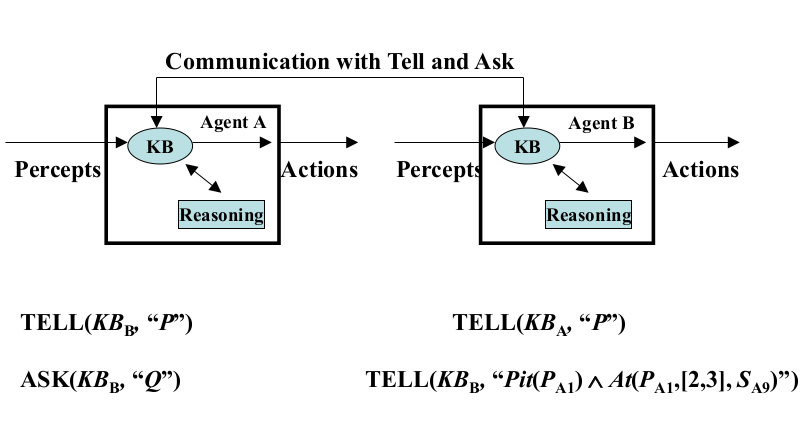
\includegraphics[scale=0.3]{img/tell and ask.png}
			\end{center}
			\item Kommunikation unter Verwendung von \textbf{Formalen Sprachen}: Agenten machen keine Annahmen über die interne Repräsentation der Sprache; Agenten teilen eine gemeinsame Sprache für die Kommunikation.
			\begin{center}
				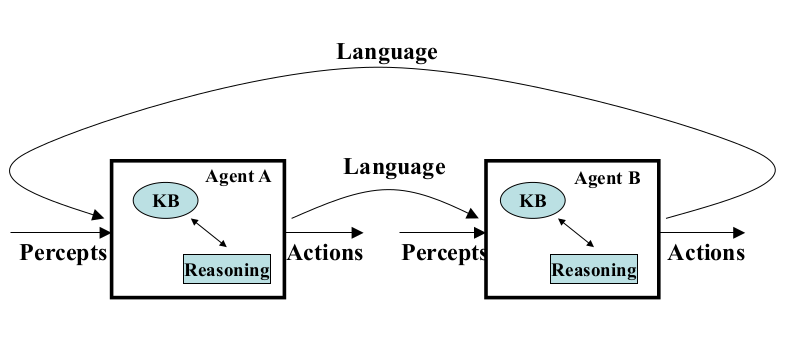
\includegraphics[scale=0.3]{img/formalLanguage.png}
			\end{center}
		\end{itemize}
		\item Größtes Problem: Kommunikation ist zweideutig; Lösung unter Berücksichtigung des Kontextes und der vorigen Kommunikationen
		\item Definition der Semantik auf Basis von Planung: bestimmte Prädikate, die in der jeweiligen precondition-delete-add Listen verwaltet werden
		\item Beispiel: request(s,h,$\phi$)
		\begin{itemize}
			\item pre: s glaubt h kann $\phi$ tun; s glaubt h glaubt h kann $\phi$; s glaubt s will $\phi$
			\item post: h glaubt s glaubt s will $\phi$
		\end{itemize}
	\end{itemize}
	\subsection{KQML und KIF}
	\begin{itemize}
		\item Nun Betrachtung von Agent Communication Languages (ACLs) d.h. dem Standardformat für den Austausch von Nachrichten
		\item Bekannteste ACL: KQML (Knowledge Query and Manipulation Language)
		\item Zwei Bestandteile: Wissens-Abfrage und -Manipulations Sprache (KQML) und Wissens-Austausch Format (KIF)
		\item KQML ist eine äußere Sprache, die verschiedene akzeptierbare Verben (performatives) definiert (Bsp: ask-if, perform, tell, reply)
		\item KIF (knowledge interchange format)ist eine Sprache für die Repräsentation des Nachrichteninhaltes (meistens ähnlich zu Common Lisp)
		\item Für die Kommunikation müssen die Agenten das gleiche Verständnis von Ausdrücken haben (Was bedeutet Schalter1?), formale Definition in einer Ontologie
	\end{itemize}
	\subsection{FIPA}
	\begin{itemize}
		\item Neue Entwicklung der Agenten Standards incl. ACL
		\item Basisstruktur ist ähnlich zu KQML: Permative + Housekeeping + Content
		\item INFORM und REQUEST sind die zwei Standard Permative in FIPA; der Rest wird auf Basis dieser definiert
		\item Bedeutung von INFORM und REQUEST hat zwei Parts: pre-condition (muss wahr sein damit der Speech Act erfolgreich ist), rational effect (Ziel, das der Sender der Nachricht erreichen möchte)
		\item Beschreibung der pre-condtions usw als logischer Ausdruck
	\end{itemize}
	\subsection{Ontologien}
	\begin{itemize}
		\item Situation: Service Oriented Computing
		\item Alle Teilnehmer haben ein gemeinsames, gleiches Verständnis von Begriffen über einer Domäne (Ontologie) d.h. jeder Teilnehmer weiß genau, was unter einem bestimmten Begriff zu verstehen ist
		\item Eine Ontologie beschreibt Begriffe und deren Relationen zu einander
		\item Ontologien unterstützen die Interaktion. Dadurch, dass sie Begriffen eine Bedeutung geben
		\item Ontologie-Sprachen erlauben dem Nutzer eine explizite und formale Kozeptionierung der Domäne
		\item Problem: je umfangreicher die Sprache desto schwieriger wird es aus diesen zu schließen
		\item Schließen in einer Ontologie
		\begin{itemize}
			\item Klassenzugehörigkeit: Wenn x in der Klasse C und C eine Unterklasse von D, ist x auch in der Klasse D
			\item Klassenäquivalenz: Wenn Klasse A ist äquivalent zu B und B zu C denn ist A äquivalent zu C
			\item Konsistenz: Wir haben X Instanzen von A und B aber  A und B sind disjunkt d.h. Fehler in der Ontologie
			\item Klassifikation: gegeben Eigenschaft-Werte-Paare für Klasse A, wenn x die Kriterien erfüllt ist x in A
		\end{itemize}
		\item Schließen ist wichtig für: Überprüfung der Ontologie und des Wissens; Überprüfung, ob ungewollte Beziehungen der Klassen entstanden sind; automatische Zuordnung von Instanzen zu Klassen
		\item Überprüfungen sind wertvoll für: den Entwurf von großen Ontologien mit mehren Autoren; Integration und Verteilung anderer Ontologien an/von verschieden Quellen
	\end{itemize}
	\section{Wie sollten Agenten kommunizieren? Strategien und Protokolle}
	\subsection{Einführung}
	\begin{itemize}
		\item Kommunikation ist wichtig für die Verteilung von Aufgaben(Aufteilung von Teilaufgaben) und Ergebnissen (Teilergebnisse)
		\item Protokolle regeln die Interaktion zwischen Agenten
	\end{itemize}
	\subsection{Contract Net}
	\begin{itemize}
		\item Realisierung von Multi-Cast Kommunikation in Agenten-basierten Systemen
		\item Zwei Rollen: Selector und Contractor
		\item Contract Net: Aufgabenverteilungs-Protokoll für Aufgabenzuweisung
		\item Schritte:
		\begin{enumerate}
			\item Recognition: Feststellung des Problems
			\item Announcement: Mitteilung des Problems an alle Teilnehmer
			\item Bidding: Teilnehmer antworten mit den erwarteten Kosten
			\item Awarding: Auftragsgeber teilt einem Teilnehmer die Aufgabe zu
			\item Expediting: Ausführung
		\end{enumerate}
		\item Recognition
		\begin{itemize}
			\item Agent nimmt Problem wahr
			\item Agent hat Ziel und merkt, dass er das Ziel nicht alleine erreichen kann (Nicht genügend Kapazität) bzw. dass er dieses Ziel nicht alleine erreichen möchte (Deadline, Lösungsqualität)
		\end{itemize}
		\item Announcement
		\begin{itemize}
			\item Agent sendet Aufgabe incl. Spezifikation der Aufgabe an alle Teilnehmer
			\item Spezifikation beinhaltet: Aufgabenbeschreibung, Anforderungen (Deadlines, Qualität der Lösung), Meta-Informationen
			\item Announcement ist ein Broadcast
		\end{itemize}
		\item Bidding
		\begin{itemize}
			\item Agenten empfangen Announcement und entscheiden sich, ob sie für die Aufgabe bieten möchten
			\item Faktoren: Agent muss entscheiden, ob er in der Lage ist die Aufgabe zu bewältigen; Agent muss die Contraints ermitteln ggf. Preis
			\item Wenn Agent mitbieten möchte, sendet er ein Gebot (tender) an Aufgabensteller
		\end{itemize}
		\item Awarding \& Expediting
		\begin{itemize}
			\item Aufgabensteller muss aus den Geboten auswählen und entscheiden wer belohnt werden soll
			\item Ergebniss wird den teilnehmenden Agenten mitgeteilt
			\item Erfolgreicher Contractor (Teilnehmer) führt die Aufgabe aus
			\item Ggf. Erweiterung der Contractor Beziehung um weitere Unterbeziehungen: sub-contracting
		\end{itemize}
		\item Problem: Spezifikation von ...
		\begin{itemize}
			\item Aufgaben: gemeinsame Sprache der Agenten
			\item Lösungsqualität: Anforderungen (Ontologien), Werbungen und Reputation
			\item Auswahl von konkurrierenden Angeboten: Präferenzen
		\end{itemize}
	\end{itemize}
	\section{Verhandlungen}
	\subsection{Einführung}
	\begin{itemize}
		\item Wie können Agenten eine Übereinkunft treffen, wenn sie sich egoistisch verhalten?
		\item Worst-Case: Null-Summen-Spiele d.h. keine Übereinkunft möglich, ABER meistens besteht eine Möglichkeit zum Treffen einer kurzzeitigen Übereinkunft - zum allgemeinen Interesse.
		\item Fähigkeiten der Verhandlung notwendig
		\item Verhandlungen werden durch einen Mechanismus (Protokoll) gesteuert
		\item Mechanismus = Regeln für das Treffen von Agenten
		\item Mechanismus-Design: Entwicklung von Mechanismen mit bestimmten Eigenschaften
		\item Mechanismus-Design Eigenschaften:
		\begin{itemize}
			\item Konvergenz und garantierter Erfolg
			\item Maximierung des Gemeinwohles
			\item Pareto-Effizienz
			\item Individuelle Rationalität
			\item Stabilität
			\item Einfachheit
			\item Verteilung
		\end{itemize} 
	\end{itemize}
	\subsection{Verhandlung - Auktionen}
	\begin{itemize}
		\item Auktionen finden zwischen einem Auktionator und einer Menge von Bietern statt
		\item Ziel: Auktionator möchte eine Zuweisung von Gütern (Ressourcen) an einen Bieter erreichen
		\item Meistens möchte Auktionator den maximalen Preis erreichen, die Bieter den minimalen
		\item Auktions-Parameter
		\begin{itemize}
			\item Güter haben: Privaten Wert, Allgemeinen Wert, Korrelierten Wert
			\item Gewinnermittelung durch: erstes Gebot, zweites Gebot
			\item Gebote sind: für alle sichtbar (open cry); verborgen (sealed bid)
			\item Gebotsabgabe: einmalig (one shot), aufsteigend, absteigend
		\end{itemize}
	\end{itemize}
	\subsubsection{Englische Auktion}
	\begin{itemize}
		\item Höchstes Gebot gewinnt, für alle sichtbar, aufsteigend
		\item Dominante Strategie: minimale Erhöhung des höchsten Gebotes bis Obergrenze erreicht, falls diese überschritten: Rückzug
		\item Anfällig: Fluch des Gewinners (Bezahlt meistens zu viel), Lockvögel (Agent arbeitet mit Auktionator zusammen und treibt den Preis künstlich in die Höhe)
	\end{itemize}
	\subsubsection{Holländische Auktion}
	\begin{itemize}
		\item Offene Gebote, absteigend
		\item Auktionator startet mit hohen Startgebot
		\item Auktionator senkt den Preis, bis ein Agent ein Gebot zu dem Preis abgibt
		\item Gewinner: Agent mit der Preisabgabe
	\end{itemize}
	\subsubsection{First-Price Sealed-Bid Auction}
	\begin{itemize}
		\item Einmaliges verborgenes Gebot
		\item Eine Runde
		\item Bieter sendet Gebot
		\item Bieter mit höchstem Gebot gewinnt
		\item Gewinner bezahlt Preis des höchstem Gebotes
		\item Beste Strategie: biete weniger als den eigentlichen Wert
	\end{itemize}
	\subsubsection{Vickrey Auction}
	\begin{itemize}
		\item Second preis, sealed bit
		\item Gewinner mit dem höchstem Gebot zum Preis vom zweit-höchstem Gebot
		\item Beste Strategie: Preisabgabe zum wirklichen Wert
		\item Überbieten wird dominiert durch das Bieten des echten Wertes
%TODO Was willst du mir sagen??
		\item[$\rightarrow$] Wenn ein Bieter mit einem höheren Wert als die anderen gewinnt, hat dieser wohl überboten; wenn Bieter eines niedrigeren Wertes als andere Bieter antritt, hat er verloren obwohl überboten hat oder nicht
		\item Unterbieten wird dominiert durch Bieten des echten Wertes
		\item[$\rightarrow$] Wenn ein Bieter zu gering bietet verliert er; wenn ein Bieter zu hoch bietet wird er gewinnen
		\item Anfällig für antisoziales Verhalten
		\begin{itemize}
			\item Agent A beziffert den Wert bei 90\$ und weiß, dass Agent B 100\$ bieten würde.
			\item Agent A kann Zuschlag also nicht bekommen.
			\item Stattdessen bietet Agent A 99\$ um den Preis für Agent B in die Höhe zu treiben und diesem so zu schaden.
		\end{itemize}
	\end{itemize}
	\subsection{Probleme}
	\begin{itemize}
		\item Auktionen sind anfällig für Lügen vom Auktionator und Absprache von Bietern
		\item Alle Auktionen sind können durch Absprache der Bieter manipuliert werden 
		\item Ein böser Auktionator kann bei der Vickrey Auktion bezüglich es zweit höchsten Gebots lügen
		\item Shills (Lockvögel) können bei der Englischen Auktion den Preis in die Höhe treiben
		\item Anwendung von Auktionen: Lastverteilung, Routing, Koordination
	\end{itemize}
	\subsection{Heterogene und selbst-motivierende Agenten}
	\begin{itemize}
		\item Kein zentrales Design
		\item Es gibt keinen globalen Nutzen
		\item Sind Dynamisch d.h. neue Typen von Agenten können leicht hinzugefügt werden
		\item Agenten sind nicht wohlwollend solange sie es nicht sein wollen d.h. Agenten kooperieren erst, wenn es nötig ist
		\item Notwendig: Entwickler einigen sich auf Standards, wie Agenten in Domäne zu agieren haben
		\item Abstimmung von Möglichkeiten und Tradeoffs für Protokolle, Strategien und die sozialen Regeln der Agenten
		\item Eigenschaften von Standards:
		\begin{itemize}
			\item Effizienz: Pareto Optimal
			\item Stabil: kein Grund vom optimal abzuweichen
			\item Einfach: gerade Berechnungs- und Kommunikationskosten
			\item Verteilt: kein zentraler Koordinator
			\item Symmetrisch: jeder Agent spielt äquivalente Rolle
		\end{itemize}
		\item MAS: Gruppe von Nutzen-maximierende heterogenen Agenten, die koexistieren in der gleichen Umgebung, evtl. Konkurrenz
		\item Auktionen als Verhandlungsmechanismus für die Teilung von Ressourcen
		\item In Abhängigkeit von Auktion wählt jeder Agent eine andere Strategie
		\item Möglich: andere Szenarien für Verhandlungen außer die Verteilung von Ressourcen
	\end{itemize}
	\subsection{Verschiedene Domänen}
	\begin{itemize}
		\item Aufgaben orientierte Domäne: Agenten wollen Aufgaben erledigen $\rightarrow$ Aufgabenverteilung
		\item Zustand orientierte Domäne: Ziele sind bestimmte finale Zustände der Welt $\rightarrow$ gemeinsamen Plan
		\item Wert orientierte Domäne: Zustände haben einen Wert $\rightarrow$ gemeinsamen Plan- und Ziel-Realisierung
	\end{itemize}
	\subsection{Aufgaben orientierte Domäne}
	\begin{itemize}
		\item Tripe: $<T,Ag,c>$
		\item T ist eine endliche Menge von möglichen Aufgaben
		\item $Ag=\{1,\dots,n\}$ ist eine Menge von beteiligten Agenten
		\item $c = p(T) \rightarrow R^+$ definiert die Kosten für die Ausführung jeder Teilmenge von Aufgaben (p ist Potenzmenge)
		\item Ein Encounter ist eine Menge von Aufgaben: $<T_1,\dots,T_n>$ mit $T_i \subseteq T$ für jedes $i \in Ag$
		\item Bestandteile: Domäne, Verhandlungsprotokoll, Verhandlungsstrategie
		\item Gegeben ein Encounter, dann ist $<T_1,T_2>$ ein Deal für die Zuweisung $T_1 \cup T_2$ bezüglich der Agenten 1 und 2
		\item Die Kosten für den Agenten i eines Deals: $\beta = <D_1,D_2>$ ist $c(D_i)$ (nachfolgend als $cost_i(\beta)$)
		\item Utility eines Deals $\beta$ des Agenten i ist mit $c(T_i)$ die ursprüngliche Zuweisung einer Aufgabe für Agent i: $utility_i(\beta) = c(T_i)-cost_i(\beta)$
		\item Conflict deal $\Omega$ ist ein Deal $<T_1,T_2>$ mit der ursprünglichen Zuweisung an Aufgaben: $utility_i(\Omega) = 0, \forall i \in Ag$
		\item Ein Deal ist individuell rational, wenn dieser den conflict deal schwach dominiert
		\item Agenten nutzen Produkt-maximierende Verhandlungsprotokolle
		\item The Monotonic Concession Protocol ???
		\begin{itemize}
			\item Verhandlung in Runden
			\item Runde 1: Agenten schlagen gleichzeitig einen Deal aus dem Verhandlungsset vor
			\item Übereinkunft, wenn ein Agent einen Deal findet, der mindestens so gut ist wie die von anderen vorgeschlagenen
			\item Wenn keine Übereinkunft nächste Runde
			\item In Runde $u+1$ darf kein Agent einen schlechteren Deal machen als der in der vorigen Runde
			\item Wenn nach einigen Runden keine Übereinkunft gefunden wird: Dann wird die Verhandlung mit dem Conflict-Deal beendet
		\end{itemize}
		\item Zeuthen Strategie ???
		\begin{itemize}
			\item Verhandlung mit dem Ziel der Messung der Bereitschaft ein Risiko einzugehen
			\item Höhere Bereitschaft, wenn der Unterschied zwischen dem aktuellen Vorschlag und dem Konfliktdeal gering ist
			\item Erster Vorschlag: Der beste Deal eines Agenten
			\item Jede Runde wird ein Agent riskieren
			\item Agenten kommen sich nur soviel entgegen, bis das Risiko erreicht ist
		\end{itemize}
	\end{itemize}
	\section{Trust and Reputation}
	\subsection{Einführung}
	\begin{itemize}
		\item Trust: Der Glaube, dass ein anderer Agent eine Aktion tun wird, ohne dass explizite Garantien vergeben werden, um ein Ziel in einer riskanten Situation zu erreichen.
		\item Reputation: Was andere Agenten bezüglich seines Verhaltens sagen
		\item Reputation erlaubt die Bildung von Trust und hat so eine soziale Komponente, die nicht nur für einen Agenten sondern für alle nützlich ist.
		\item Jeder Agent wird durch andere Agenten beobachtet, keine zentrale Autorität
		\item Subjective vs. Globale Reputation
		\begin{itemize}
			\item Subjektiv: Jeder Agent hat eine eigene Vorstellung von der Reputation anderer Agenten
			\item Global: Reputation als eine zentrale Ressource, auf die alle Agenten Zugriff haben und die gleichen Reputationswerte erhalten.
			\item Vorteil global: Reputation ist auch für neue Agenten verfügbar; einfacher für Agenten, da diese Werte nicht berechnet werden müssen
			\item Nachteil global: Funktioniert nur unter der Annahme, dass alle Agenten denken und sich ähnlich verhalten, da interne Zustände des Agenten nicht berücksichtigt werden; Es ist nicht immer erwünscht, dass Agenten Information public machen oder diese an eine zentrale Verwaltungsstelle senden
			\item Ein hoher Trust in die zentralen Organisation ist notwendig
		\end{itemize}
		\item Vgl. Ebay: komplett zentral, Käufer hinterlassen Kommentare + Bewertung nach Käufen, jeder Teilnehmer hat einen Wert als Summe der Bewertungen
		\item Beispiel: Regret System
	\end{itemize}
	\subsection{Regret System}
	\begin{center}
		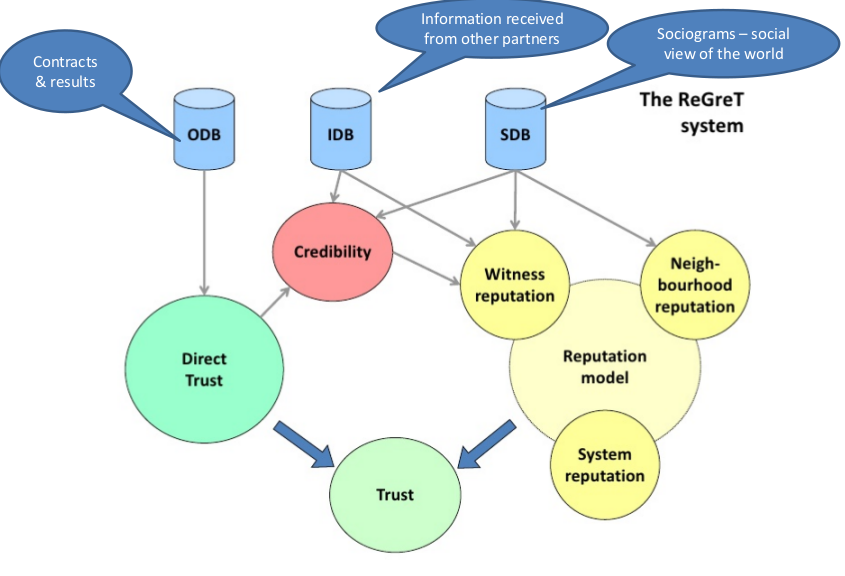
\includegraphics[scale=0.3]{img/regret.png}
	\end{center}
	\begin{itemize}
		\item Modulares Trust und Reputations-System für komplexe E-Commerce Umgebungen, in denen soziale Relationen zwischen den Teilnehmern eine wichtige Rolle spielen
		\item Outcome: Initialer Vertrag + Realisierung des Partners (Attribute: Lieferungstag, Kosten, Qualität, Quantität)
		\item Impression: Subjekte Auswertung des Outcomes
		\item ??? Wie detailliert ???
	\end{itemize}
	\section{Blackboard}
	\subsection{Allgemein}
	\begin{itemize}
		\item Indirekte Kommunikation, d.h. keine direkte Kommunikation zwischen den Agenten sondern über ein Medium
		\item Kommunikation durch Schreiben der Information auf ein Blackboard (zentraler Datenspeicher)
		\item Agenten können partielle Lösungen für das Problem dort veröffentlichen
		\item Zentrale Datenstruktur ist Flaschenhals und muss ggf. über irgendwelche Hierarchien verfügen
		\item Subscripe-notify Pattern: Agent bekundet Interesse an  bestimmen Ereignissen, wenn ein Ereignis eintritt, wird der Agent benachrichtigt (proaktiv)
		\item Annahmen: verschiedene Agenten greifen asynchron auf die Datenstruktur zu; ????
		\item Wissensquelle: Agent drückt ein Teil der Lösung aus; ???
		\item (??? IRG WAS MIT PRECONDITIONS ???)
		\item Verschiedene Hierarchien für Tests (??? PRECONDITIONS ???)
%TODO Wofür steht WQ?
		\item Modularität: Man kann einzelne WQ des Systems entwickeln, ohne zu wissen welche anderen WQ es gibt (also indirekte Kommunikation)
		\item Interessant: Wie verändert sich die Systemleistung durch Austausch einzelner WQ?
		\item Kommunikation:
		\begin{enumerate}
			\item Sammlung von Daten über Events für zukünftige Anwendung
			\item Detektion von Ereignissen, die vorigen Annahmen widersprechen (???)
		\end{enumerate}
		\item Lokale Kontexte: Jeder hat ein eigenes lokalen Abbild der Datenbank, die von Interesse ist, Übertragung neuer Events an entsprechende Interessierte
		\item (??? Folie übersprungen zu Integrität ???)
		\item Jeder Agent hat eine eigene Datenbank, Verteilung der Information über Blackboard; lokale Datenbanken bilden zusammen eine globale Datenbank
	\end{itemize}
	\subsection{Alternative Architekturen}
	\begin{itemize}
		\item Beispiel: Speech Understanding,
		\item Ansatz 1: Pipe-and-Filter Architektur; Problem: keine klare Trennung, ggf Wissen aus unterschiedlichen Quellen notwendig d.h. Architektur wird unnötige komplex
		\item Ansatz 2: Object-Orientierte-Architektur; Problem: nicht flexibel da jede WQ wissen muss, was eine andere WQ produzieren kann; Lösung: Client-Broker Ansatz aber recht komplex
		\item Ansatz 3: Sichten-System; Problem: 
		\item Besser: Alle Prozesse kommunizieren über Blackboard, Ziel: Wissensverteilung der Partiellen Lösungen
	\end{itemize}
	\section{Organisationskontrolle}
	\subsection{Allgemein}
	\begin{itemize}
		\item Organisationskontrolle (Wer kann mit wem interagieren) kann Kommunikation und Kooperation vereinfachen (kürzere Entscheidungshierarchie, weniger Kommunikation)
		\item Strukturierung als zentrale Aufgabe reflektiert die Aufgabe und sorgt für eine effizientere Lösung der Aufgabe
		\item Organisationstrolle funktioniert, wenn ein Problem zerlegbar und häufig wiederholbar ist
		\item Framework für die Skalierung der Aufgaben
		\item Ziel: Wissen lokal zu halten, damit nicht zusätzlicher Aufwand durch Verwaltung fremden Wissens entsteht
		\item Organisations Tradeoff
	\end{itemize}
	\section{Agenten und Mobilität}
	\begin{itemize}
		\item Verteilte Orte: Wie können diese miteinander reden?
		\item Verteilte Systeme: verschiedene Möglichkeiten um Methoden von anderen Koten (Remote Procedure Call) aufzurufen
		\item Lösungen: Stub, Skeleton. Marshalling (Serialisierung von Objekten), IDL
		\item Stub hat Referenz zu Skeleton-Methodes
		\item Probleme: 
		\begin{itemize}
			\item Client kann blockieren
			\item Verbindung kann nicht sicher sein (fällt ggf aus), Implementierung von Timeouts usw (unreliable links)
			\item Übertragung von großen Daten kann ein Problem sein. Es ist besser, wenn der Server Berechnungen mit Daten vornimmt - ohne zu verschicken ABER möglicherweise kennt der Server den Algorithmus nicht (Lösung: Mobile Agents)
		\end{itemize}
		\item Agenten-basierter Ansatz: Alternative zu RPC ist RP
		\item Client macht Code für Prozeduren und Klassen bekannt
		\item Prozedur + Aktuellen Zustand präsentiert einen Mobiler Agent
		\item Weak migration: ? (standard)
		\item Strong migration: ?
		\item Remote Programming: Konventionen zwischen Client und Server für Befehle und Datentypen bilden eine Sprache
	\end{itemize}
\end{document}